
\documentclass[calculator,datasheet,sample]{exam}
%\documentclass[calculator,refrigeranttables,psychrometricchart,airtables,datasheet]{exam}


% The full list of class options are
% calculator : Allows approved calculator use.
% datasheet : Adds a note that data sheet are attached to the exam.
% handbook : Allows the use of the engineering handbook.
% resit : Adds the resit markings to the paper.
% sample : Adds conspicuous SAMPLE markings to the paper
% solutions : Uses the contents of \solution commands (and \solmarks) to generate a solution file
\usepackage{pdfpages}
\usepackage{lscape,comment}

\coursecode{EG5597}%
\coursetitle{Advanced Chemical Engineering}%
%\coursecode{EG3539}%
%\coursetitle{Thermodynamics}%

\examtime{00.00--00.00}%
\examdate{00}{05}{2015}%
\examformat{Candidates must attempt \textit{all} questions.}

\newcommand{\frc}{\displaystyle\frac}
\newcommand{\br}[1]{\!\left( #1 \right)}
\newcommand{\abs}[1]{\left| #1 \right|}
\newcommand{\fracd}[2]{\frac{\mathrm{d} #1}{\mathrm{d} #2}}
\newcommand{\fracp}[2]{\frac{\partial #1}{\partial #2}}
\renewcommand{\d}[1]{\mathrm{d} #1 }
\newcommand{\Ma}{\mathrm{M\!a}}

\begin{document}


%%%
%%% Question 01 
%%%
\begin{question}
\begin{enumerate}
\item  An oil export pump requires 2200 kW of power. This is provided by a coupled gas turbine which has a thermal efficiency of the turbine is 34$\%$. The power losses between the turbine and the pump are 5 $\%$. The turbine is fuelled by methane with a calorific value of 55500 kJ/kg. Calculate the mass of carbon dioxide that the turbine will discharge if it is operating for 20 years? The molecular weight of methane and CO2 are 16 and 44 respectively.~\marks{5}

\item Describe a simple cycle, a combined cycle and a combined heat and power gas turbine system. Sketches may help.~\marks{9}

\item A gas turbine rating chart is shown in the attached figure. What full load power output would be achieved at an air temperature of 15$^{\circ}$C? What is the machine efficiency at these conditions? What full load output could be achieved if the air temperature is increased to 30$^{\circ}$C. What is the machine efficiency at 15 and 30$^{\circ}$C. Explain the difference in efficiency at the two air temperatures.~\marks{6}
\begin{center}
\includegraphics[width=10.0cm,height=12.0cm]{./Pics/EG5597_Sample_Pic1.pdf}
\end{center}

\end{enumerate}
\end{question}


%%%
%%% Question 01 
%%%
\begin{question} In an air-standard Otto cycle, the isentropic compression and expansion strokes are replaced by polytropic processes -- $PV^{\gamma}=\text{constant}$, with $\gamma=1.3$,
\begin{itemize}
\item {\bf 1--2:} Polytropic compression;
\item {\bf 2--3:} Addition of heat at constant volume;
\item {\bf 3--4:} Polytropic expansion and;
\item {\bf 4--1:} Rejection of heat at constant volume. 
\end{itemize}
The compression ratio $\left(\frc{V_{1}}{V_{2}}=\frc{V_{4}}{V_{3}}\right)$ is 9 for the modified cycle. At the beginning of compression, $P_{1}=1.0\;\text{bar}$ and $T_{1}=300K$. The maximum temperature during the cycle is $2000K$. 
\begin{enumerate}
\item In Table \ref{exam2_table1}, determine {\it (a)-(g)}.~\marks{7}
\begin{table}[h]
\begin{center}
\begin{tabular}{|| c | c c c c || }
\hline\hline
        & {\bf $P$ (bar)} & {\bf $T$ (K)}  & {\bf V$\left(m^{3}/kg\right)$} & {\bf $U\;\left(kJ/kg\right)$} \\
{\bf 1} & 1               &     300        &       (a)                      & (b)                 \\    
{\bf 2} & --              &     (c)        &       --                      &  (d)                 \\
{\bf 3} & --              &    2000        &       --                       & (e)                 \\
{\bf 4} & --              &    (f)         &       --                      &  (g)                 \\
\hline\hline
\end{tabular}
\end{center}
\caption{Thermodynamic table of the modified air-standard Otto cycle.}\label{exam2_table1}
\end{table}
%
\solution{The modified air-standard Otto cycle with the following initial conditions:
\begin{displaymath}
\gamma = 1.3,\;\;\; \frc{V_{1}}{V_{2}}=\frc{V_{4}}{V_{3}}=9, \;\;\; P_{1}= 1\;\text{bar}, \;\;\; T_{1}=300\;K, \;\;\; T_{\text{max}}=T_{4}=2000\;K
\end{displaymath}

In order to fill Table \ref{exam2_table1}, we need to calculate all relevant variables for each stage of the cycle (using the ideal-gas properties of air table):
\begin{enumerate}
\item {\bf Stage 1:} At $T_{1}=300\;K\text{ and }P_{1}=1\text{ bar }\;\Rightarrow\;U_{1}=214.07\frc{kJ}{kg}$. From the ideal gas equation,~\solmarks{2/7}
\begin{displaymath}
V_{1}=\frc{R T_{1}}{P_{1}}= 0.8610 \frc{m^{3}}{kg}
\end{displaymath}
\item {\bf Stage 2:} $T_{2}=T_{1}\left(\frc{V_{1}}{V_{2}}\right)^{\gamma-1}=300\left(9\right)^{0.3}=580K \Rightarrow U_{2}=419.55\frc{kJ}{kg}$~\solmarks{2/7}
\item {\bf Stage 3:} $T_{3}=2000\;K\;\Rightarrow\;U_{3}=1678.7\frc{kJ}{kg}$;~\solmarks{1/7}
\item {\bf Stage 4:} $T_{4}=T_{3}\left(\frc{V_{3}}{V_{4}}\right)^{\gamma-1}=1034.57\; K \Rightarrow U_{4}=788.67\frc{kJ}{kg}$~\solmarks{2/7}
\end{enumerate}

\begin{table}[h]
\begin{center}
\begin{tabular}{|| c || c |c |c |c || }
\hline\hline
        & {\bf $P$ (bar)} & {\bf $T$ (K)}  & {\bf V$\left(m^{3}/kg\right)$} & {\bf $U\;\left(kJ/kg\right)$} \\
\hline
{\bf 1} & 1               &     300        &  (a)0.8610                    & (b)214.07                 \\    
{\bf 2} & --              & (c)580         &       --                      & (d)419.55                 \\
{\bf 3} & --              &    2000        &       --                      & (e)1678.7                 \\
{\bf 4} & --              & (f)1034.57     &       --                      & (g)788.67                 \\
\hline\hline
\end{tabular}
\end{center}
\caption{Thermodynamic table of the modified air-standard Otto cycle.}\label{exam2_table1}
\end{table}
}


%
\item Calculate the mass-based heat $\left(Q/m\right)$ and work $\left(W/m\right)$ (both in $kJ/kg$) for each stroke in the cycle;~\marks{8}
%
\solution{
For each stroke $i--j$:
\begin{enumerate}
%
\item {\bf 1--2:}~\solmarks{2/8}
\begin{eqnarray}
&& \frc{W_{12}}{m}=\int_{1}^{2}P dV = \frc{R\left(T_{2}-T_{1}\right)}{1-\gamma} = -267.85 \frc{kJ}{kg} \nonumber \\
&& \frc{Q_{12}}{m}=\left(U_{2}-U_{1}\right)+\frc{W_{12}}{m}=-62.37\frc{kJ}{kg} \nonumber
\end{eqnarray}

% 
\item {\bf 2--3:}~\solmarks{2/8}
\begin{eqnarray}
&& \frc{W_{23}}{m}=0  \nonumber \\
&& \frc{Q_{23}}{m}=\left(U_{3}-U_{2}\right)+\frc{W_{23}}{m}=1259.15\frc{kJ}{kg} \nonumber 
\end{eqnarray} 

%
\item {\bf 3--4:}~\solmarks{2/8}
\begin{eqnarray}
&& \frc{W_{34}}{m}=\int_{3}^{4}P dV = \frc{R\left(T_{4}-T_{3}\right)}{1-\gamma} = 923.10 \frc{kJ}{kg} \nonumber \\
&& \frc{Q_{34}}{m}=\left(U_{4}-U_{3}\right)+\frc{W_{34}}{m}=33.07\frc{kJ}{kg} \nonumber 
\end{eqnarray}

% 
\item {\bf 4--1:}~\solmarks{2/8}
\begin{eqnarray}
&& \frc{W_{41}}{m}=0 \nonumber \\
&& \frc{Q_{41}}{m}=\left(U_{4}-U_{1}\right)+\frc{W_{41}}{m}=-574.60\frc{kJ}{kg} \nonumber 
\end{eqnarray} 

\end{enumerate}

}
%

\item Calculate the thermal efficiency;~\marks{3}
\begin{displaymath}
\eta = \frc{\left(W_{\text{cycle}}/m\right)}{\left(Q_{\text{in}}/m\right)}
\end{displaymath}
%
\solution{~\solmarks{3/3}
\begin{eqnarray}
&& \frc{W_{\text{cycle}}}{m} = \frc{W_{12}}{m} + \frc{W_{34}}{m} = 655.25\frc{kJ}{kg} \nonumber \\ 
&& \frc{Q_{in}}{m} = \frc{Q_{23}}{m} + \frc{Q_{34}}{m} = 1292.22\frc{kJ}{kg} \nonumber \\
&& \eta = \frc{655.25}{1292.22}=0.507 \nonumber 
\end{eqnarray}

}
%

\item Calculate the mean effective pressure (in bar).~\marks{2}
\begin{displaymath}
\text{MEP} = \frc{\left(W_{\text{cycle}}/m\right)}{V_{1}-V_{2}}
\end{displaymath}
%
\solution{~\solmarks{2/2}
\begin{displaymath}
\text{MEP} = \frc{\left(W_{\text{cycle}}/m\right)}{V_{1}-V_{2}}=\frc{\left(W_{\text{cycle}}/m\right)}{V_{1}\left(1 - \frc{V_{2}}{V_{1}}\right)} = 8.56\text{ bar}
\end{displaymath}

}
%
\end{enumerate} 
Also given:
\begin{itemize}
\item Isentropic relations for ideal gas:
\begin{eqnarray}
&& TV^{\gamma-1}=\text{constant} \nonumber \\
&& TP^{\frac{1-\gamma}{\gamma}}=\text{constant} \nonumber \\
&& PV^{\gamma}=\text{constant} \nonumber 
\end{eqnarray}
\item Molecular weight of air:  $MW=28.97\frc{kg}{kgmol}$;
\item Polytropic relation for an ideal gas from state $i$ to $j$:
\begin{displaymath}
\frc{W_{ij}}{m} = \int_{i}^{j}P dV = \frc{R\left(T_{j}-T_{i}\right)}{1-\gamma}
\end{displaymath}
\end{itemize}
\end{question}


\clearpage


%%%
%%% Question 2 
%%%
\begin{question} A vapour-compression refrigeration cycle is operated with Refrigerant R-134a as working fluid. Saturated vapour enters the compressor (with isentropic efficiency of 80$\%$) at $2$ bar, and saturated liquid exits the condenser at $8$ bar. The mass flow rate of R-134a is $7$ kg/min.
\begin{enumerate}
\item Sketch the schematic of the cycle indicating the numbering used in the calculation;~\marks{2}
%
\solution{Figure. \ref{Ex02:Q04}.~\solmarks{2/2}
\begin{figure}[h]
\label{Ex02:Q04}
\begin{center}
\includegraphics[width=8.0cm,height=8.0cm]{./Pics/Exam_Refrigeration4}
\vspace{-1.9cm}
\caption{Schematic of the vapour compression refrigeration cycle.}
\end{center}
\end{figure}
}
%
\item Calculate all enthalpies in the cycle $\left(H_{k}\;\forall k\in\left\{1,2,3,4\right\}\right)$;~\marks{8}
%
\solution{

\begin{itemize}
\item {\bf Stage 1:} Saturated vapour at $P_{1}=2\text{ bar} \Rightarrow$ $H_{1}=241.30\frc{kJ}{kg}$ and $S_{1}=0.9253\frc{kJ}{kg.K}$;~\solmarks{2/8}
\item {\bf Stage 2:} Isentropic compression $\left(S_{2s}=S_{1}\right)$ at $P_{2}=P_{3}=8\text{ bar}$. At this pressure, the entropy of the saturated vapour is $S_{g}=0.9066\frc{kJ}{kg.K} << S_{2s}$, therefore we can conclude that the fluid is at superheated state $\Rightarrow$ (via linear interpolation) $T_{2s}=36.59^{\text{o}}C$ and $H_{2s}=269.92\frc{kJ}{kg}$. Now, in order to calculate $H_{2}$,~\solmarks{2/8}
\begin{displaymath}
\eta_{C}=\frc{H_{2s}-H_{1}}{H_{2}-H_{1}}\;\Rightarrow\; H_{2}=277.08\frc{kJ}{kg}
\end{displaymath}
\item {\bf State 3:} Saturated liquid at $P_{3}=8\text{ bar} \Rightarrow$ $H_{3}=93.42\frc{kJ}{kg}$;~\solmarks{2/8}
\item {\bf State 4:} Isenthalpic expansion: $H_{4}=H_{3}$.~\solmarks{2/8}
\end{itemize}
}
%

\item Calculate the compressor power $\left(W_{\text{C}}\right)$ in $kW$;~\marks{2}
%
\solution{~\solmarks{2/2}
\begin{displaymath}
W_{\text{C}}=\dot{m}_{R}\left(H_{2}-H_{1}\right) = 4.17\text{ kW}
\end{displaymath}
}
%
\item Determine the refrigeration capacity $\left(R_{\text{n}}\right)$ in {\it tons};~\marks{2}
%
\solution{~\solmarks{2/2}
\begin{displaymath}
R_{\text{n}}=\dot{m}_{R}\left(H_{1}-H_{4}\right) = 4.93\text{ tons}
\end{displaymath}
}
%
\item Calculate the coefficient of performance of the cycle $\left(\text{COP}=R_{\text{n}}/W_{\text{C}}\right)$;~\marks{2}
%
\solution{~\solmarks{2/2}
\begin{displaymath}
\text{COP}= \frc{W_{\text{C}}}{R_{\text{n}}}= 4.13
\end{displaymath}
}
%
\item Sketch the $TS$ diagram, indicating all stages of the cycle.~\marks{4}
%
%\solution{See Figure \ref{ExQ03b}~\solmarks{4/4}
\solution{See Figure 2~\solmarks{4/4}
\begin{figure}[!h]
\begin{center}
\includegraphics[width=8.0cm,height=6.0cm]{./Pics/Exam_Refrigeration4_TS}
\label{ExQ03b}
\vspace{-.4cm}
\caption{$TS$ diagram for the vapour compression refrigeration cycle.}
\end{center}
\end{figure}
}
%
\end{enumerate}

The efficiency of the compressor can be expressed as,
\begin{displaymath}
\eta_{C}=\frc{H_{ks}-H_{k-1}}{H_{k}-H_{k-1}} 
\end{displaymath}
where $H_{ks}$ is the ideal enthalpy of the flow at stage $k$.

\end{question}

\clearpage



%%%
%%% Question 5
%%%
\begin{question} 
\begin{enumerate}%[(1)]
\item Saturated refrigerant R-134a vapour at $P_{1}=400\;kPa$ is compressed by a piston to $P_{2}=16\;\text{bar}$ in a reversible adiabatic process. Critical pressure and temperature of R-134a are 4.059 MPa and 101.06$^{\text{o}}$C.
\begin{enumerate}[(a)]
\item Calculate the work done by the piston;\marks{6}
%
\solution{In order to calculate the work executed by the piston we need to calculate teh thermodynamic variables at states $1$ and $2$.
\begin{enumerate}
%
\item {\bf State 1:} Saturated vapour at $P_{1}=400$ kPa = 4 bar $\Rightarrow$ $T_{1}=T_{\text{sat}}=8.93^{\text{o}}C$, $V_{1}=V_{g}=0.0509\frc{m^{3}}{kg}$, $H_{1}=252.32\frc{kJ}{kg}$, $S_{1}=0.9145\frc{kJ}{kg.K}$ and \\
$U_{1}=231.97\frc{kJ}{kg}$~\solmarks{2/6}. 
%
\item {\bf State 2:} Adiabatic (i.e., isentropic) compression to $P_{2}=16$ bar $\Rightarrow$ $S_{2}=S_{1}=0.9145\frc{kJ}{kg.K}$. At this pressure, the saturated vapour entropy is smaller than the prescribed entropy, i.e., $S_{g}=0.8982\frc{kJ}{kg.K}<<S_{2}$. Therefore, the fluid in $2$ is at superheated state, thus (via linear interpolation): $T_{2}=61.96^{\text{o}}C<<T_{C}$, $V_{2}=0.01254\frc{m^{3}}{kg}$, $H_{2}=280.77\frc{kJ}{kg}$ and \\
$U_{2}=260.71\frc{kJ}{kg}$~\solmarks{2/6}.\\
 Notice that $P_{2} << P_{C}$ and $V_{2} << V_{1}$. 
%
\end{enumerate}
 Now, from the First Law:~\solmarks{2/6}
\begin{displaymath}
dU = dQ + dW \Rightarrow U_{2}-U_{1} = 0 + \Delta W \Rightarrow \Delta W = 28.74 \frc{kJ}{kg}
\end{displaymath}
}
%
\item Sketch the $TS$ and $PV$ diagrams including the constant pressure and temperature lines.~\marks{4}
\solution{Figure \ref{Ex02:Q05}. ~\solmarks{4/4}
\begin{figure}[!h]
\begin{center}
\includegraphics[width=12.0cm,height=8.0cm]{./Pics/Exam_PV-TS_Diagrams}
\vspace{-1.7cm}
\caption{$TS$ and $PV$ (rhs) diagrams.}\label{Ex02:Q05}
\end{center}
\end{figure}
}
\end{enumerate}

\item A reciprocating engines was designed to operate with the following stages:
\begin{itemize}
\item 1--2: Isentropic compression;
\item 2--3: Addition of heat at constant volume;
\item 3--4: Addition of heat at constant pressure;
\item 4--5: Isentropic expansion and;
\item 5--1: Rejection of heat at constant volume.
\end{itemize}
\begin{enumerate}
\item Sketch the {\it TS} and {\it PV} diagrams for this cycle;~\marks{4}
%
\solution{This is a dual combustion cycle and the $TS$ and $PV$ diagrams are shown in Fig. \ref{Ex01:Q05}.~\solmarks{4/4}
\begin{figure}[h]
\begin{center}
\includegraphics[width=12.0cm,height=8.0cm]{./Pics/InternalCombustion_IdealDualCombustion}
\vspace{-1.7cm}
\caption{Dual combustion cycle -- $PV$ and $TS$ (rhs) diagrams.}\label{Ex01:Q05}
\end{center}
\end{figure}
}
%
\item For this cycle, define an expression for the net work $\left(W_{\text{net}}\right)$ as a function of mass of air ($m$), heat capacities $\left(C_{p}\text{ and } C_{v}\right)$ and temperatures $\left(T_{j}\right)$,~\marks{6}
\begin{displaymath}
W_{\text{net}}= W_{\text{net}}\left(m,C_{p},C_{v},T_{j}\right)=\text{Heat Supplied} - \text{Heat Rejected}
\end{displaymath}
%
\solution{Thermal analysis, for $m$ kg of air:
\begin{enumerate}%[(a)]
\item Total heat supplied (2--3 + 3--4): $m\left[C_{v}\left(T_{3}-T_{2}\right) + C_{p}\left(T_{4}-T_{3}\right)\right]$~\solmarks{2/6}
\item Total heat rejected (5--1): $mC_{v}\left(T_{5}-T_{1}\right)$~\solmarks{2/6}
\item Net Work: $W_{\text{net}}= m\left[C_{v}\left(T_{3}-T_{2}\right) + C_{p}\left(T_{4}-T_{3}\right)-C_{v}\left(T_{5}-T_{1}\right)\right]$~\solmarks{2/6}
\end{enumerate}

}
%
\end{enumerate}


\end{enumerate}


\end{question}


\clearpage

%%%%%%%%%%%%%%%%%%%%%%%%%%
%%%% Question 01       %%%
%%%%%%%%%%%%%%%%%%%%%%%%%%
%\begin{question}
%\begin{enumerate}[(a)]
%%%%%%%%%%%%%%%%%%%%%%%%%%%
%\item ~\marks{3}
%\solution{
%}
%
%%%%%%%%%%%%%%%%%%%%%%%%%%%
%\item ~\marks{3}
%\solution{
%}
%\end{enumerate}
%\end{question}
%
%\clearpage
%
%%%%%%%%%%%%%%%%%%%%%%%%%%
%%%% Question 02       %%%
%%%%%%%%%%%%%%%%%%%%%%%%%%
%\begin{question} 
%\begin{enumerate}[(a)]
%%%%%%%%%%%%%%%%%%%%%%%%%%%
%\item ~\marks{3}
%\solution{
%}
%
%%%%%%%%%%%%%%%%%%%%%%%%%%%
%\item ~\marks{3}
%\solution{
%}
%\end{enumerate}
%\end{question}
%\clearpage
%
%%%%%%%%%%%%%%%%%%%%%%%%%%
%%%% Question 03       %%%
%%%%%%%%%%%%%%%%%%%%%%%%%%
%\begin{question} 
%\begin{enumerate}[(a)]
%%%%%%%%%%%%%%%%%%%%%%%%%%%
%\item ~\marks{3}
%\solution{
%}
%
%%%%%%%%%%%%%%%%%%%%%%%%%%%
%\item ~\marks{3}
%\solution{
%}
%\end{enumerate}
%\end{question}
%
%\clearpage


%%%%%%%%%%%%%%%%%%%%%%%%%
%%% Question 04       %%%
%%%%%%%%%%%%%%%%%%%%%%%%%
\begin{question} 
\begin{enumerate}[(a)]
%%%%%%%%%%%%%%%%%%%%%%%%%%
\item Energy conservation in a steady flow device implies
\begin{align*}
 \dot{Q} - \dot{W}_s = \dot{m} \left(h_2 + \frac{u_2^2}{2} + g z_2\right) - \dot{m} \left(h_1 + \frac{u_1^2}{2} + g z_1\right),
\end{align*}
where $\dot{Q}$ is the rate of heat addition, $\dot{W}_s$ is the rate of shaft work done by the fluid, $h$ is the specific enthalpy and $u$ is the fluid velocity. Briefly explain the physical significance of the fluxes making up the right-hand side of this equation. \marks{3}
\solution{Enthalpy flux $\dot{m} h$, kinetic energy flux $\dot{m} u^2/2$ and potential energy flux $\dot{m} g z$. \solmarks{3/3}}

%%%%%%%%%%%%%%%%%%%%%%%%%%
\item An ideal gas flows through a steady flow device at a rate of $3$\,kg/s, and does work on a set of compressor blades at a rate of $28$\,kW. The gas has a temperature of $60^\circ$C when it enters the device through a circular inlet of diameter $50$\,cm (where the flow properties are denoted by a subscript 1) and exits the device at $50^\circ$C through a circular outlet of diameter $20$\,cm (where the flow properties are denoted 2). The inlet and outlet are at the same vertical height, while the pressure at the inlet is $100$\,kPa. Assuming no heat is added or removed from the device, then determine:

\begin{enumerate}[i)]
\item The inlet and outlet velocities; \marks{9}
\solution{The density of the fluid at the inlet is
\begin{align*}
 \rho_1 = \frac{p_1}{R T_1} = \frac{100000}{300 \times (60 + 273.15)} = 1.000550\,\mbox{kg/m}^3
\end{align*}~\solmarks{1/9}


The inlet and outlet areas are
\begin{align*}
 A_1 = \frac{\pi d_1^2}{4} =& \frac{\pi \times 0.5^2}{4} = 0.196350\,\mbox{m}^2, \\
 A_2 = \frac{\pi d_2^2}{4} =& \frac{\pi \times 0.2^2}{4} = 0.031416\,\mbox{m}^2.
\end{align*}~\solmarks{2/9}

The inlet velocity can now be obtained from the mass flux
\begin{align*} 
 u_1 = \frac{\dot{m}}{\rho_1 A_1} = \frac{3}{1.000550 \times 0.196350} = 15.270471\,\mbox{m/s}.
\end{align*}~\solmarks{1/9}

The outlet velocity can be obtained from the SFEE, which can be written in the form
\begin{align*}
 u_2 = \sqrt{2 \left[c_p \left(T_1 - T_2\right) + \frac{u_1^2}{2} - \frac{\dot{W}_s}{\dot{m}}\right]} = 39.57930\,\mbox{m/s},
\end{align*}
where we've used the fact the gas is an ideal gas and written $h = c_p T$. \solmarks{5/9}
}

\item The pressure at the outlet. \marks{2}
\solution{The density at the outlet can be obtained from the mass flux
\begin{align*}
 \rho_2 = \frac{\dot{m}}{u_2 A_2} = 2.412700\,\mbox{kg/m}^3.
\end{align*}\solmarks{1/2}

The pressure at the outlet can subsequently be obtained from the ideal gas law
\begin{align*}
 p_2 = \rho_2 R T_2 = 233899.2\,\mbox{Pa}.
\end{align*}\solmarks{1/2}
}
\end{enumerate}

You may assume the specific heat capacity of the gas $c_p = 1000$\,J/(kg K) and the specific gas constant $R=300$\,J/(kg K).


%%%%%%%%%%%%%%%%%%%%%%%%%%
\item Downstream of the compressor, the gas flows isentropically into a difuser. Explain what is meant by an isentropic flow.~\marks{2}
\solution{A flow at constant entropy OR $\d{s}=0$.\solmarks{2/2}}

%%%%%%%%%%%%%%%%%%%%%%%%%%
\item Isentropic flow along a diffuser satisfies the equation
\begin{align*}
 \frac{1}{1 - \Ma^2} \frac{1}{A} \fracd{A}{x} = \frac{1}{\rho u^2} \fracd{p}{x} = -\frac{1}{u} \fracd{u}{x}.
\end{align*}
With reference to this equation, explain how the pressure $p$, and flow velocity $u$ vary if gas flows subsonically along the diffuser. \marks{4}
\solution{In a diffuser $\fracd{A}{x} > 0$.\solmarks{1/4}

For subsonic flow $\Ma < 1$ and hence $1 - \Ma^2 > 0$. \solmarks{1/4}

$A > 0$, $\rho>0$ and $u>0$, so $\fracd{p}{x}$ has the same sign as $\fracd{A}{x}$ and therefore the pressure increases with flow along a subsonic diffuser. \solmarks{1/4}

$\fracd{u}{x}$ has the opposite sign to $\frac{A}{x}$ so flow velocities decrease with flow along the diffuser. \solmarks{1/4}}
\end{enumerate}
\end{question}

\clearpage

%%%%%%%%%%%%%%%%%%%%%%%%%
%%% Question 05       %%%
%%%%%%%%%%%%%%%%%%%%%%%%%
\begin{question} 
\begin{enumerate}[(a)]
%%%%%%%%%%%%%%%%%%%%%%%%%%
\item Air in an air-conditioning system is mixed adiabatically with air from outside in a steady process. If the inlets to the mixing chamber are labelled 1 and 2, and the outlet is labelled 3, then state equations corresponding to the mass conservation of dry air, the mass conservation of water vapour and the conservation of energy. Hence show that
\begin{align*}
 \frac{\dot{m}_{a_2}}{\dot{m}_{a_1}} = \frac{h_3 - h_1}{h_2 - h_3} = \frac{\omega_3 - \omega_1}{\omega_2 - \omega_3}
\end{align*}
where $\dot{m}$ is a mass flux, $h$ is a specific enthalpy and $\omega$ is a specific humidity.\marks{8}
\solution{
In the mixing section
\begin{align*}
\mbox{\textit{Conservation of dry air:}} & & \dot{m}_{a_1} + \dot{m}_{a_2} = \dot{m}_{a_3}, \\
\mbox{\textit{Conservation of water vapour:}} & & \dot{m}_{a_1} \omega_1 + \dot{m}_{a_2} \omega_2 = \dot{m}_{a_3} \omega_3, \\
\mbox{\textit{Conservation of energy:}} & & \dot{m}_{a_1} h_1 + \dot{m}_{a_2} h_2 = \dot{m}_{a_3} h_3.
\end{align*}~\solmarks{3/8}

Using the dry air mass conservation equation to eliminate $\dot{m}_{a_3}$ from the other two expressions, gives
\begin{align*}
 \dot{m}_{a_1} \omega_1 + \dot{m}_{a_2} \omega_2 =& \left(\dot{m}_{a_1} + \dot{m}_{a_2}\right) \omega_3, \\
 \dot{m}_{a_1} h_1 + \dot{m}_{a_2} h_2 =& \left(\dot{m}_{a_1} + \dot{m}_{a_2}\right) h_3.
\end{align*}~\solmarks{2/8}

Collecting all the terms involving $\dot{m}_{a_2}$ on the left-hand side and all the terms involving $\dot{m}_{a_3}$ on the right-hand side gives
\begin{align*}
 \dot{m}_{a_2} \omega_2 - \dot{m}_{a_2} \omega_3 =& \dot{m}_{a_1} \omega_3 - \dot{m}_{a_1} \omega_1, \\
 \dot{m}_{a_2} h_2 - \dot{m}_{a_1} h_3 =& \dot{m}_{a_2} h_3 - \dot{m}_{a_1} h_1.
\end{align*}~\solmarks{1/8}

Rearranging
\begin{align*}
 \dot{m}_{a_2} \left(\omega_2 - \omega_3\right) =& \dot{m}_{a_1} \left(\omega_3 - \omega_1\right), \\
 \dot{m}_{a_2} \left(h_2 - h_3\right) =& \dot{m}_{a_2} \left(h_3 - h_1\right).
\end{align*}~\solmarks{1/8}

Finally
\begin{align*}
 \frac{\dot{m}_{a_2}}{\dot{m}_{a_1}} = \frac{\omega_3 - \omega_1}{\omega_2 - \omega_3}, \quad \mbox{and} \quad \frac{\dot{m}_{a_2}}{\dot{m}_{a_2}} =& \frac{h_3 - h_1}{h_2 - h_3},
\end{align*}
which gives the necessary result.\solmarks{1/8}
}

%%%%%%%%%%%%%%%%%%%%%%%%%%
\item Inlet 1 brings $25$\,m$^3$/min of saturated air from the cooling section of the air conditioning system at a temperature of 7$^\circ$C. Inlet 2 brings $40$\,m$^3$/min of air from outside with a specific humidity of 0.01\,kg water/kg dry air and a temperature of 39$^\circ$C. Assuming the mixing is adiabatic and occurs at 1\,atm, then determine:

\begin{enumerate}[i)]
\item The outlet mass flux of dry air;~\marks{4}
\solution{From the psychrometric chart the inlet gas streams (labelled 1 from the
air-conditioning system and 2 from outside), have the properties
\begin{align*}
 V_1 =& 0.8\,\mbox{m}^3 /\mbox{kg dry air}, \quad \mbox{and} \quad V_2 = 0.9\,\mbox{m}^3 /\mbox{kg dry air}.
\end{align*}~\solmarks{2/4}

The inlet mass flow rates are
\begin{align*}
 \dot{m}_{a_1} =& \frac{\dot{V}_1}{V_1} = \frac{25}{0.8} = 31.25\,\mbox{kg/min}, \\
 \dot{m}_{a_2} =& \frac{\dot{V}_2}{V_2} = \frac{40}{0.9} = 44.44444\,\mbox{kg/min}.
\end{align*}~\solmarks{1/4}

Therefore mass conservation gives the outlet of mass flux of dry air to be
\begin{align*}
 \dot{m}_{a_3} = \dot{m}_{a_1} + \dot{m}_{a_2} = 75.694444\,\mbox{kg/min}.
\end{align*}~\solmarks{1/4}
}


%%%%%%%%%%%%%%%%%
\item The specifc humidity of the mixture;~\marks{5}
\solution{From the psychrometric chart
\begin{align*}
 \omega_1 =& 0.006\,\mbox{kg water}/\mbox{kg dry air}.
\end{align*}\solmarks{1/5}

Now using the result from part (a),
\begin{align*}
 \frac{\dot{m}_{a_2}}{\dot{m}_{a_1}} = \frac{\omega_3 - \omega_1}{\omega_2 - \omega_3}.
\end{align*}
Rearranging
\begin{align*}
 \left(1 + \frac{\dot{m}_{a_2}}{\dot{m}_{a_1}}\right)\omega_3 = \omega_1 + \omega_2 \frac{\dot{m}_{a_2}}{\dot{m}_{a_1}}.
\end{align*}\solmarks{2/5}

Now
\begin{align*}
 \frac{\dot{m}_{a_2}}{\dot{m}_{a_1}} = \frac{44.44444}{31.25} = 1.42222222222,
\end{align*}
which gives
\begin{align*}
 \omega_3 =& 0.008386\,\mbox{kg water}/\mbox{kg dry air}.
\end{align*}\solmarks{2/5}
}

%%%%%%%%%%%%%%%
\item The relative humidity and the dry-bulb temperature.~\marks{3}
\solution{The remain properties are determined by the intersection of straight line joining 1 and 2, and the $\omega_3 = 0.008386$\,kg water/kg dry air. \solmarks{1/3}

This gives
\begin{align*}
 \phi_3 =& 35\%, \quad \mbox{and} \quad T_3 = 29^\circ\mbox{C}.
\end{align*}~\solmarks{2/3}

}
\end{enumerate}
\end{enumerate}
\end{question}

\clearpage

\vfill

\paperend

%\begin{comment}
\begin{landscape}
\begin{center}
\includegraphics[width=1.5\textwidth]{./Pics/PsychrometricChart}
\end{center}
\end{landscape}
{

  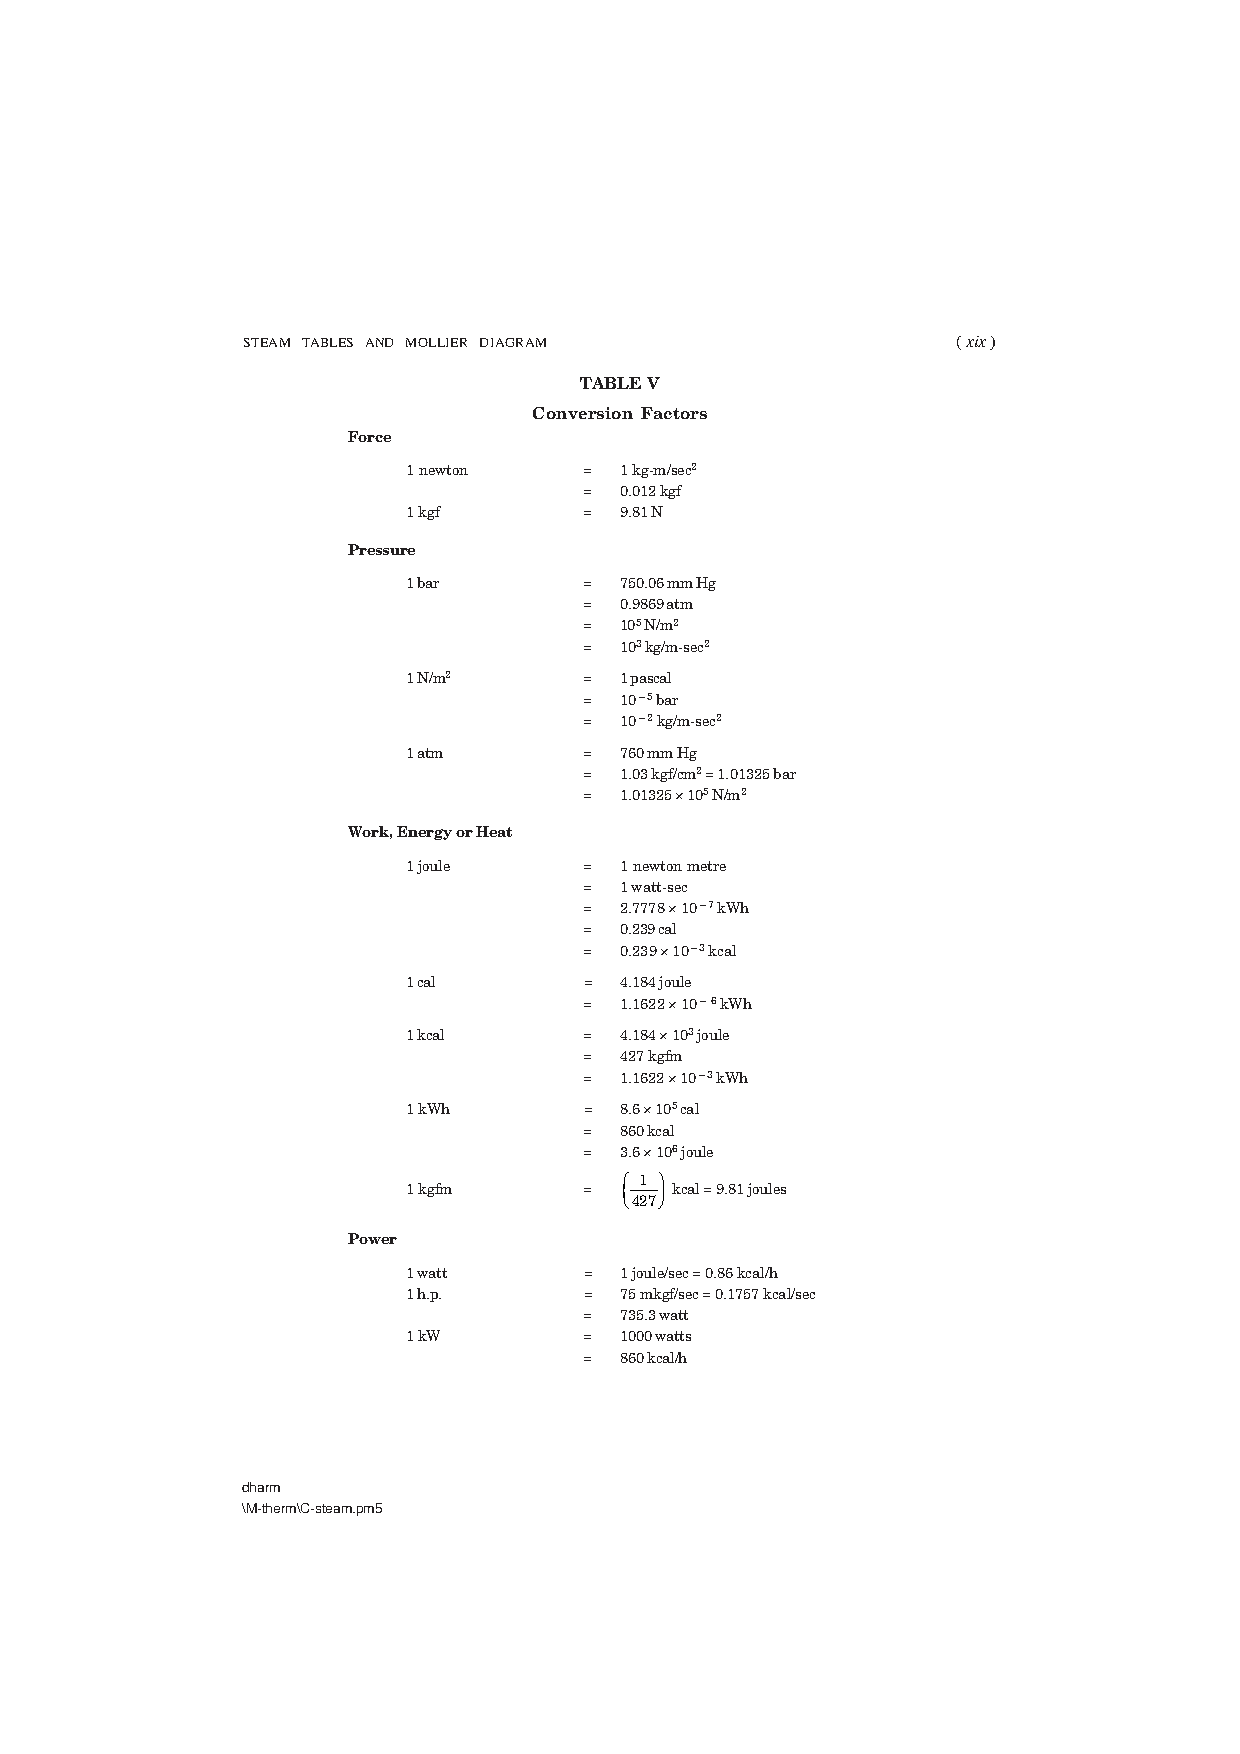
\includepdf[pages=-,fitpaper]{./Pics/UnitsConversion}
  \includepdf[pages=-,fitpaper]{./Pics/AirTable}
  %\includepdf[pages=-,fitpaper]{SteamTable_2}
  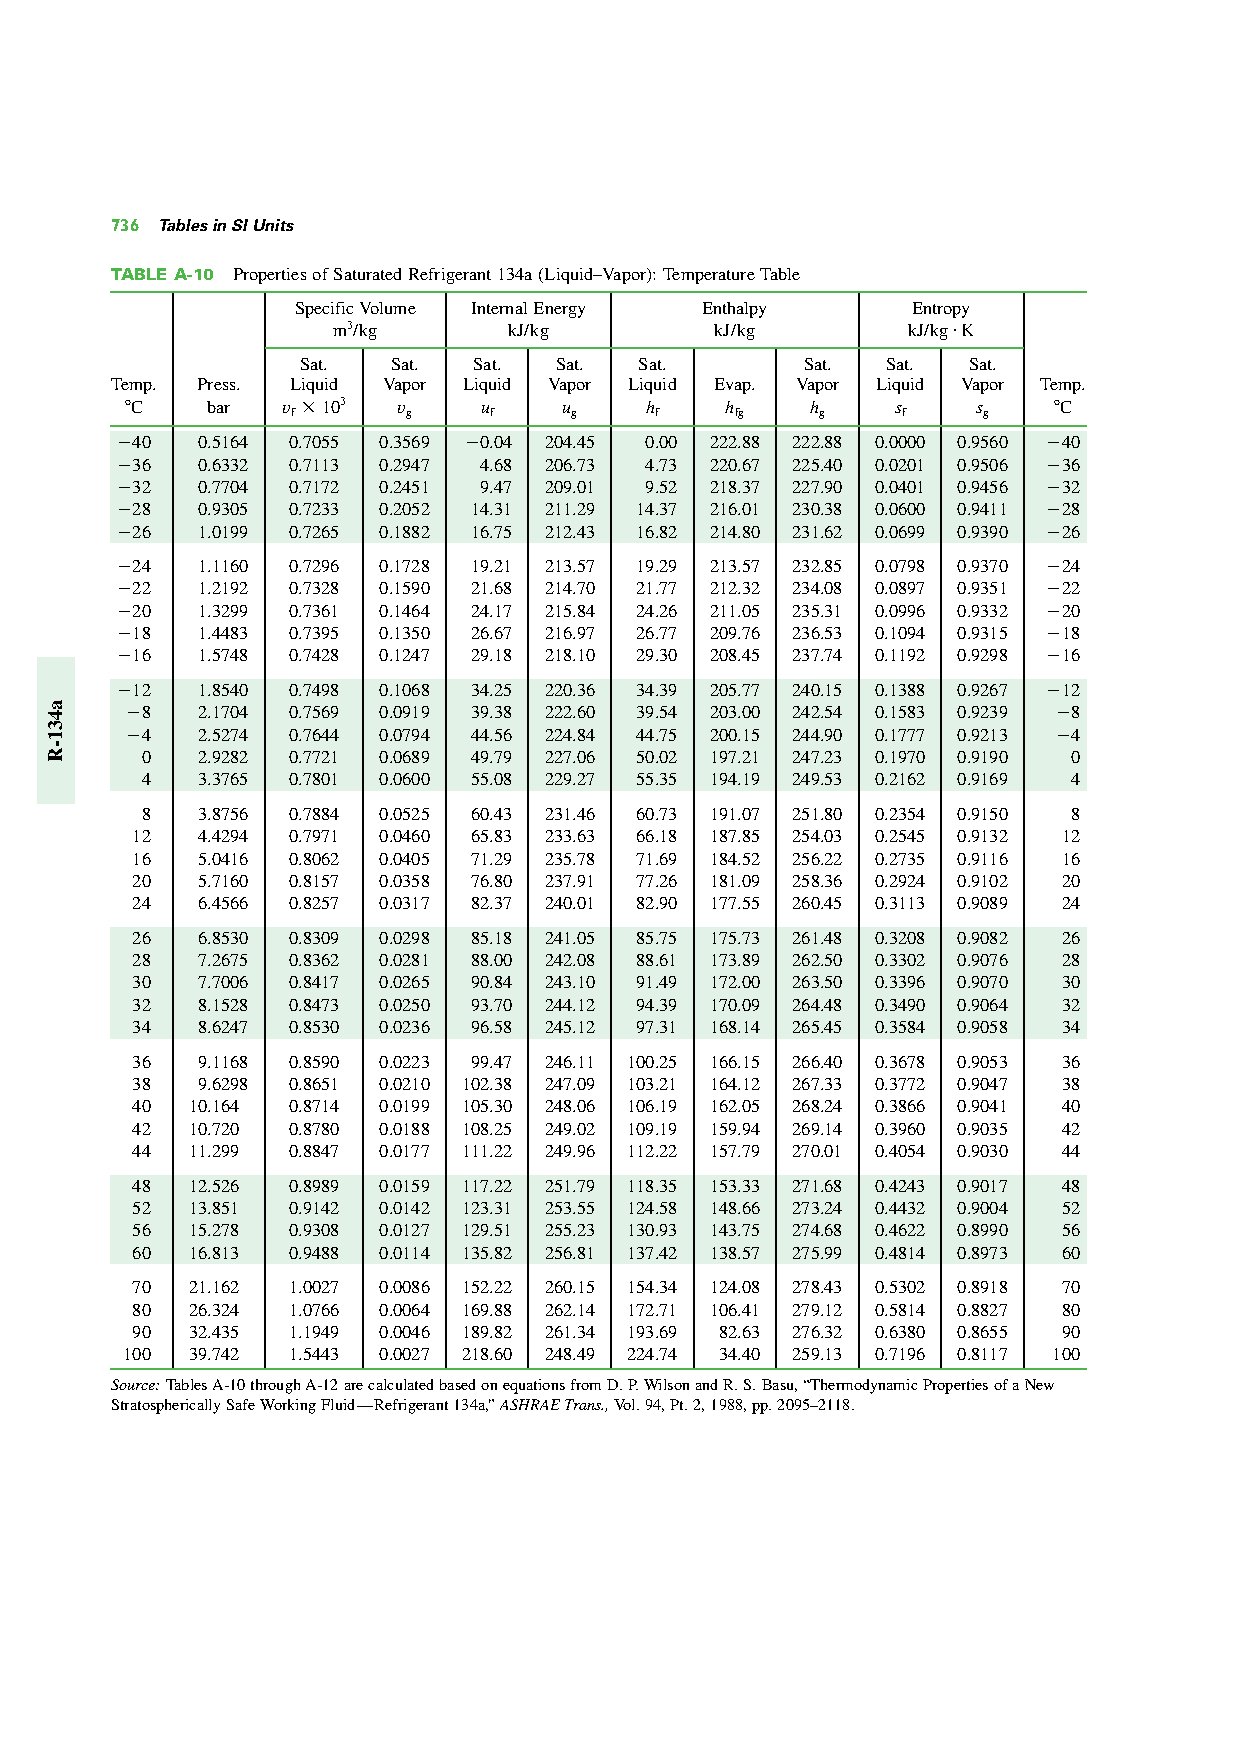
\includepdf[pages=-,fitpaper]{./Pics/Tables_R134}
}

%\end{comment}


\end{document}
